\documentclass[12pt,a4paper,oneside]{article}

\usepackage[italian]{babel}
\usepackage[T1]{fontenc}
\usepackage[utf8]{inputenc}
\usepackage[margin=1in]{geometry}
\usepackage{graphicx}

\usepackage[
	linesnumbered,
	ruled,
	italiano
]{algorithm2e}

\begin{document}
	
	\title{N-bodies simulation\\Assignment programmazione concorrente e distribuita}
	\author{Filippo Barbari}
	\date{}%no date
	\maketitle
	
	\tableofcontents
	\newpage
	
	\section{Analisi}
	\subsection{Descrizione della simulazione}
	Questa simulazione è una variante della nota "simulazione di $N$ corpi". La simulazione è composta da:
	\begin{itemize}
		\item un numero $N$ di corpi ciascuno dotato di massa ma incorporeo (non ha una dimensione)
		\item un dominio bidimensionale finito di forma rettangolare e allineato con gli assi cartesiani
		\item una forza repulsiva tra i corpi (descritta in dettaglio di seguito)
		\item una forza d'attrito applicata sui singoli corpi
	\end{itemize}
	
	\subsection{Analisi dell'algoritmo}
	\begin{algorithm}
		\SetAlgorithmName{Algoritmo}{}{}
		\KwIn{B, array dei corpi}
		\KwIn{bounds, i bordi della simulazione}
		\KwIn{steps, numero di iterazioni da calcolare}
		
		\For{$steps$ times}{
			\ForEach{Body $b$ in $B$}{
				computeTotalForces($b$)\;
			}
			\ForEach{Body $b$ in $B$}{
				computeAcceleration($b$)\;
				updateVelocity($b$)\;
				updatePosition($b$)\;
				checkAndSolveBoundaryCollisions($b$)\;
			}
		}
		\caption{N-Bodies simulation}
	\end{algorithm}
	
	\subsection{Analisi delle dipendenze tra dati}
	Questo algoritmo presenta due dipendenze molto importanti:
	\begin{itemize}
		\item il risultato di una determinata iterazione $i > 0$ dipende dal risultato dell'iterazione $i-1$
		\item il risultato dell'aggiornamento dei parametri di un qualsiasi corpo $b_i$ (accelerazione, velocità e posizione) dipende dal risultato del calcolo di tutte le forze repulsive agenti su $b_i$
	\end{itemize}
	
	\section{Design}
	\subsection{Mutua esclusione}
	Come emerso dall'analisi dell'algoritmo, non è necessario l'utilizzo di alcun meccanismo di mutua esclusione per evitare letture e scritture concorrenti sui dai dei singoli corpi. Difatti, è sufficiente \textbf{partizionare} l'array globale dei corpi in tante porzioni quanti sono i thread utilizzati, ognuno dei quali si occuperà di aggiornare solamente i corpi della propria partizione.
	
	\subsection{Sincronizzazione}
	Un problema più importante consiste, invece, nella \textbf{sincronizzazione} dei thread al fine di non violare nessuna delle due dipendenze tra dati individuate. Per fare ciò utilizziamo due Barrier, ovvero dei costrutti che permettono la sincronizzazione globale dei thread, come riportato nello pseudocodice di seguito. Le Barrier utilizzate sono implementate nella classe \texttt{nbodies.utils.barrier.ReusableBarrier}.
	
	\begin{algorithm}
		\SetAlgorithmName{Algoritmo}{}{}
		\KwIn{B, array dei corpi}
		\KwIn{bounds, i bordi della simulazione}
		\KwIn{steps, numero di iterazioni da calcolare}
		
		partition($B$)\;
		\For{$steps$ times}{
			\ForEach{Body $b$ in $B$}{
				computeTotalForces($b$)\;
			}
			barrier()\;
			\ForEach{Body $b$ in $B$}{
				computeAcceleration($b$)\;
				updateVelocity($b$)\;
				updatePosition($b$)\;
				checkAndSolveBoundaryCollisions($b$)\;
			}
			barrier()\;
		}
		\caption{Parallel N-Bodies simulation}
	\end{algorithm}

	\subsection{GUI}
	Per evitare un eccessivo overhead della GUI, ho scelto di renderla completamente asincrona rispetto alla simulazione.
	
	\section{Dettagli implementativi}
	Per evitare \textit{overhead} non necessari e per semplificare il codice, ogni \texttt{Worker}, prima di cominciare il ciclo vero e proprio, estrae dalla lista dei corpi una lista di puntatori ai corpi su cui deve operare.
	
	\section{Valutazione prestazioni}
	\subsection{Tempi di esecuzione}
	I tempi riportati di seguito fanno riferimento ad un'esecuzione parallela che utilizza 8 thread.
	
	\hfill
	\begin{minipage}{.4\textwidth}
		Senza GUI
		
		\begin{tabular}{|l|l|l|}
			\hline
			\multicolumn{1}{|c|}{\textbf{N. corpi}} & \multicolumn{1}{c|}{\textbf{N. step}} & \multicolumn{1}{c|}{\textbf{Tempo}} \\ \hline
			100 & 1000 & 0,11 \\ \hline
			100 & 10000 & 0,602 \\ \hline
			100 & 50000 & 2,939 \\ \hline
			1000 & 1000 & 1,403 \\ \hline
			1000 & 10000 & 14,139 \\ \hline
			1000 & 50000 & 65,73 \\ \hline
			5000 & 1000 & 47,193 \\ \hline
			5000 & 10000 & 474,334 \\ \hline
			5000 & 50000 & 2351,408 \\ \hline
		\end{tabular}
	\end{minipage}
	\hfill
	\begin{minipage}{.4\textwidth}
		Con GUI
		
		\begin{tabular}{|l|l|l|}
			\hline
			\multicolumn{1}{|c|}{\textbf{N. corpi}} & \multicolumn{1}{c|}{\textbf{N. step}} & \multicolumn{1}{c|}{\textbf{Tempo}} \\ \hline
			100 & 1000 & 0,117 \\ \hline
			100 & 10000 & 0,74 \\ \hline
			100 & 50000 & 3,364 \\ \hline
			1000 & 1000 & 3,101 \\ \hline
			1000 & 10000 & 30,25 \\ \hline
			1000 & 50000 & 143,894 \\ \hline
			5000 & 1000 & 68,841 \\ \hline
			5000 & 10000 & 673,219 \\ \hline
			5000 & 50000 & 3328,55 \\ \hline
		\end{tabular}
	\end{minipage}
	\hfill

	\subsection{Speedup}
	Valori speedup (misurati con 1000 corpi e 10000 step).
	
	\hfill
	\begin{minipage}{.45\textwidth}
		\centering
		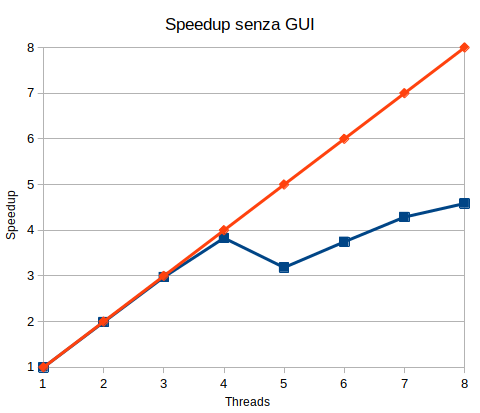
\includegraphics[width=\linewidth]{speedup-no-gui}
		\label{fig:speedup-no-gui}
	\end{minipage}
	\hfill
	\begin{minipage}{.45\textwidth}
		\centering
		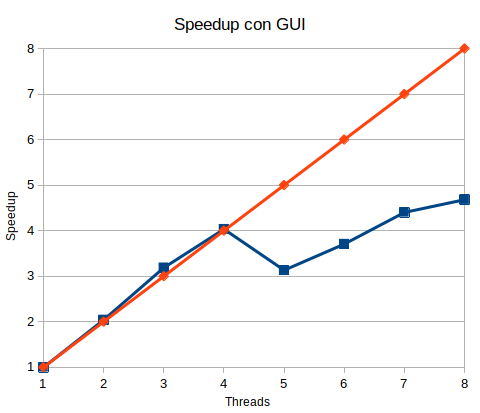
\includegraphics[width=\linewidth]{speedup-gui}
		\label{fig:speedup-gui}
	\end{minipage}
	\hfill
	
	\subsection{Strong scaling efficiency}
	\hfill
	\begin{minipage}{.45\textwidth}
		\centering
		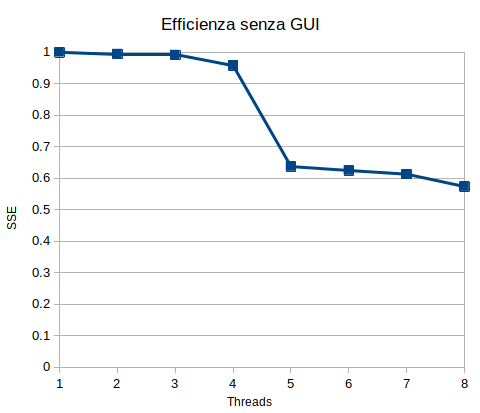
\includegraphics[width=\linewidth]{sse-no-gui}
		\label{fig:sse-no-gui}
	\end{minipage}
	\hfill
	\begin{minipage}{.45\textwidth}
		\centering
		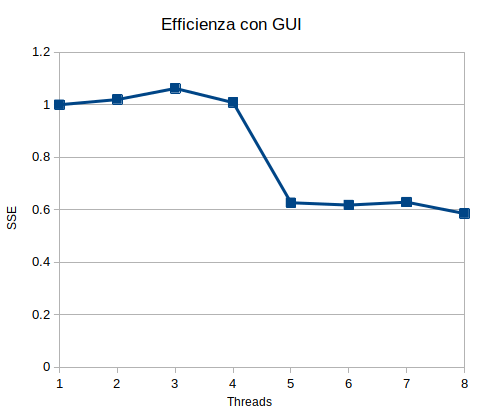
\includegraphics[width=\linewidth]{sse-gui}
		\label{fig:sse-gui}
	\end{minipage}
	\hfill
\end{document}